% This is "sig-alternate.tex" V2.1 April 2013
% This file should be compiled with V2.5 of "sig-alternate.cls" May 2012
%
% This example file demonstrates the use of the 'sig-alternate.cls'
% V2.5 LaTeX2e document class file. It is for those submitting
% articles to ACM Conference Proceedings WHO DO NOT WISH TO
% STRICTLY ADHERE TO THE SIGS (PUBS-BOARD-ENDORSED) STYLE.
% The 'sig-alternate.cls' file will produce a similar-looking,
% albeit, 'tighter' paper resulting in, invariably, fewer pages.
%
% ----------------------------------------------------------------------------------------------------------------
% This .tex file (and associated .cls V2.5) produces:
%       1) The Permission Statement
%       2) The Conference (location) Info information
%       3) The Copyright Line with ACM data
%       4) NO page numbers
%
% as against the acm_proc_article-sp.cls file which
% DOES NOT produce 1) thru' 3) above.
%
% Using 'sig-alternate.cls' you have control, however, from within
% the source .tex file, over both the CopyrightYear
% (defaulted to 200X) and the ACM Copyright Data
% (defaulted to X-XXXXX-XX-X/XX/XX).
% e.g.
% \CopyrightYear{2007} will cause 2007 to appear in the copyright line.
% \crdata{0-12345-67-8/90/12} will cause 0-12345-67-8/90/12 to appear in the copyright line.
%
% ---------------------------------------------------------------------------------------------------------------
% This .tex source is an example which *does* use
% the .bib file (from which the .bbl file % is produced).
% REMEMBER HOWEVER: After having produced the .bbl file,
% and prior to final submission, you *NEED* to 'insert'
% your .bbl file into your source .tex file so as to provide
% ONE 'self-contained' source file.
%
% ================= IF YOU HAVE QUESTIONS =======================
% Questions regarding the SIGS styles, SIGS policies and
% procedures, Conferences etc. should be sent to
% Adrienne Griscti (griscti@acm.org)
%
% Technical questions _only_ to
% Gerald Murray (murray@hq.acm.org)
% ===============================================================
%
% For tracking purposes - this is V2.0 - May 2012

\documentclass{sig-alternate-05-2015}


\begin{document}

% Copyright
\setcopyright{acmcopyright}
%\setcopyright{rightsretained}
%\setcopyright{usgov}
%\setcopyright{usgovmixed}
%\setcopyright{cagov}
%\setcopyright{cagovmixed}


%%% % DOI
%%% \doi{10.475/123_4}

%%% % ISBN
%%% \isbn{123-4567-24-567/08/06}

%Conference
\conferenceinfo{HPCSYSPROS '16}{November 14, 2016, Salt Lake City, UT, USA}

%%% \acmPrice{\$15.00}

%
% --- Author Metadata here ---
%%% \conferenceinfo{WOODSTOCK}{'97 El Paso, Texas USA}
%\CopyrightYear{2007} % Allows default copyright year (20XX) to be over-ridden - IF NEED BE.
%\crdata{0-12345-67-8/90/01}  % Allows default copyright data (0-89791-88-6/97/05) to be over-ridden - IF NEED BE.
% --- End of Author Metadata ---

\title{Cluster Computing with OpenHPC}
%%% \title{Alternate {\ttlit ACM} SIG Proceedings Paper in LaTeX
%%% Format\titlenote{(Produces the permission block, and
%%% copyright information). For use with
%%% SIG-ALTERNATE.CLS. Supported by ACM.}}
%%% \subtitle{[Extended Abstract]
%%% \titlenote{A full version of this paper is available as
%%% \textit{Author's Guide to Preparing ACM SIG Proceedings Using
%%% \LaTeX$2_\epsilon$\ and BibTeX} at
%%% \texttt{www.acm.org/eaddress.htm}}}

\numberofauthors{8}
\author{
\alignauthor Karl W. Schulz \\ \affaddr{Intel Corp.}
\alignauthor C. Reese Baird \\ \affaddr{Intel Corp.}
\alignauthor David Brayford \\ \affaddr{Leibniz Supercomputing Centre}
\and
\alignauthor Yiannis Georgiou \\ \affaddr{Atos}
\alignauthor Gregory M. Kurtzer  \\ \affaddr{Lawrence Berkeley National Laboratory}
\alignauthor Derek Simmel \\ \affaddr{Pittsburgh Supercomputing Center}
\and
\alignauthor Nirmala Sundararajan \\ \affaddr{Dell}
\alignauthor Thomas Sterling     \\ \affaddr{Indiana University}
\alignauthor Eric Van Hensbergen  \\ \affaddr{ARM}
}


\maketitle
\begin{abstract}
OpenHPC is a newly formed, community-based project
%Linux Foundation collaborative Project whose
that is providing an integrated collection of HPC-centric software
components that can be used to implement a full-featured reference HPC compute
resource. Components span the entire HPC software ecosystem including
provisioning and system administration tools, resource management, I/O
services, development tools, numerical libraries, and performance analysis
tools.

Common clustering tools and scientific libraries are distributed as pre-built
and validated binaries and are meant to seamlessly layer on top of existing
Linux distributions. The architecture of OpenHPC is intentionally modular to
allow end users to pick and choose from the provided components, as well as to
foster a community of open contribution. This paper presents an overview of the
underlying community vision, governance structure, packaging conventions, build
and release infrastructure and validation methodologies.

\end{abstract}



%
% The code below should be generated by the tool at
% http://dl.acm.org/ccs.cfm
% Please copy and paste the code instead of the example below.

\begin{CCSXML}
  <ccs2012>
  <concept>
  <concept_id>10003456.10003457.10003490.10003503</concept_id>
  <concept_desc>Social and professional topics~Software
  management</concept_desc>
  <concept_significance>500</concept_significance>
  </concept>
  <concept>
  <concept_id>10003456.10003457.10003490.10003507</concept_id>
  <concept_desc>Social and professional topics~System management</concept_desc>
  <concept_significance>300</concept_significance>
  </concept>
  <concept>
  <concept_id>10011007.10011006.10011072</concept_id>
  <concept_desc>Software and its engineering~Software libraries and
  repositories</concept_desc>
  <concept_significance>500</concept_significance>
  </concept>
  <concept>
  <concept_id>10011007.10011006.10011066</concept_id>
  <concept_desc>Software and its engineering~Development frameworks and
  environments</concept_desc>
  <concept_significance>300</concept_significance>
  </concept>
  <concept>
  <concept_id>10010520.10010521.10010537</concept_id>
  <concept_desc>Computer systems organization~Distributed
  architectures</concept_desc>
  <concept_significance>300</concept_significance>
  </concept>
  </ccs2012>
\end{CCSXML}

\ccsdesc[500]{Social and professional topics~Software management}
\ccsdesc[300]{Social and professional topics~System management}
\ccsdesc[500]{Software and its engineering~Software libraries and repositories}
\ccsdesc[300]{Software and its engineering~Development frameworks and
  environments}
\ccsdesc[300]{Computer systems organization~Distributed architectures}

%
% End generated code
%

%
%  Use this command to print the description
%
\printccsdesc

%%% \keywords{ACM proceedings; \LaTeX; text tagging}

\section{Introduction}
This guide presents a simple cluster installation procedure using components
from the Forest Peak (\FSP{}) software stack. \FSP{} represents an aggregation of a number of
common ingredients required to deploy and manage an HPC Linux* cluster including
provisioning tools, resource management, I/O clients, development tools, and a variety of
scientific libraries. These packages have been pre-built with HPC integration
in mind and represent a mix of open-source components combined with \Intel{}
development and analysis tools (e.g. \Intel{} Parallel Studio XE Cluster Edition).
%This install guide assumes availablility of a {\em master} host
%that will have access to common OS repositories and the \FSP{} repository in order
%to facilitate software installs and dependency resolution.  
The documentation herein is intended to be reasonably generic, but uses the
underlying motivation of a small, 4-node cluster install to define a step-by-step
process. Several optional customizations are included and the intent is that
these collective instructions can be modified as needed for local site
customizations. 


\section{Community building blocks for HPC systems}

\subsection{Motivation}
Many HPC sites spend considerable effort aggregating a large suite of
open-source components to provide a capable HPC environment for their users.
This is frequently motivated by the necessity to build and deploy HPC focused
packages that are either absent or outdated in popular Linux
distributions. Further, local packaging or customization typically tries to
give software versioning access to users (e.g. via environment modules or
similar equivalent).  With this background motivation in mind, combined with a
desire to minimize duplication and share best practices across sites, the OpenHPC community
project was formed with the following mission and vision principles: \\

\noindent {\bf Mission:} to 
provide a reference collection of open-source HPC software components and
best practices, lowering barriers to deployment, advancement, and use of
modern HPC methods and tools.

\noindent {\bf Vision:} OpenHPC components and best practices will enable and
accelerate innovation and discoveries by broadening access to state-of-the-art,
open-source HPC methods and tools in a consistent environment, supported by a
collaborative, worldwide community of HPC users, developers, researchers,
administrators, and vendors. \\

%%% OpenHPC
%%% is focused on lowering the barrier to entry for HPC by providing a collection
%%% of pre-packaged and validated binary components that can be used to install and
%%% manage HPC clusters throughout their life cycle. We also provide multiple
%%% system configuration recipes that leverage community reference designs and best
%%% practices.

The remaining sections provide a further overview of the community project
by highlighting related work (\S\ref{sec:related_work}), the technical governance
structure (\S\ref{sec:governance}), repository enablement (\S\ref{sec:repo_enable}), packaging
conventions~(\S\ref{sec:packaging}), underlying build
infrastructure~(\S\ref{sec:build_infra}), and integration testing~(\S\ref{sec:integ_testing}).

\newpage
\subsection{Related Work} \label{sec:related_work}

The installation, deployment and configuration of High Performance Computing clusters is a rather tedious work. 
There are various open source and proprietary cluster management tools that attempt to provide a complete solution to this problem.
In the open-source world the most widely known solutions are Rocks and OSCAR.
Rocks \cite{rocks2003,rocks_url}, an open source Linux-based cluster solution package, can significantly reduce the complexity of building HPC clusters.
It provides a specific bundle of software components covering the different administrative needs of a cluster and offers an easy to use GUI
for the different steps of the installation procedure.
All cluster services and tools are installed and configured during the initial installation of the frontend with no need to download and
manual configure other external packages. Furthermore, with the use of Rolls \cite{rolls2004} the administrator can customize the base installation of packages with
additional software that integrate seamlessly and automatically into the management and packaging mechanisms of the base software.
%It makes use of Kickstart and RPM to manage the distribution of node file system and provides component based configuration method to realize module reuse.
The latest and current stable version of Rocks, version 6.2, is based upon CentOS 6.6.

OSCAR \cite{oscar2001,oscar_url} (Open Source Cluster Application Resources) is fully integrated and easy to install software bundle designed for
high performance cluster computing. The fundamental function of OSCAR is to build and maintain clusters. 
OSCAR follows a different methodology than Rocks; once the frontend is installed and booted, the cluster building components are downloaded and installed
through tools that try to simplify the complexity of the different administrative tasks. 
There have been some variations of OSCAR based on the same framework to cover different types of cluster environments such as Thin-Oscar for diskless platforms
and HA-Oscar to support High Availability. OSCAR is supported upon various Linux distributions such as CentOS and Debian. However, even if OSCAR and its 
variations are still being used in production, the project is no longer actively maintained and the latest version 6.1.1 was released in 2011. 
%OSCAR also provides a GUI for installation and configuration purposes.
%OSCAR is based upon a virtual image of the target machine using System Installation Suite (SIS). There is also an OSCAR database (ODA) that stores cluster information, 
%a parallel distributed “shell” tool set called C3 and an environment management facility called Env-Switcher.

OpenHPC is much less automated than Rocks, does not provide a GUI interface, expects a certain expertise from the administrator,
but it offers a greater choice of software components, promoting flexibility, for each level of the software stack. Furthermore
OpenHPC is supported and maintained by a group of vendors, research centers and laboratories that have as common goal standardization through 
sharing of best practices.



\subsection{Governance \& Community} \label{sec:governance}
Under the auspices of the Linux Foundation, OpenHPC has established a two
pronged governance structure consisting of a governing board and a technical
steering committee (TSC). The governing board is responsible for budgetary
oversight, intellectual property policies, marketing, and long-term road map
guidance. The TSC drives the technical aspects of the project including stack
architecture, software component selection, builds and releases, and day-to-day
project maintenance. Individual roles within the TSC are highlighted in
Figure~\ref{fig:tsc_governance}.  These include common roles like maintainers
and testing coordinators, but also include unique HPC roles designed to ensure
influence, and capture points of view, from two key constituents. In particular,
the {\em component development representative(s)} are included to represent the
upstream development communities for software projects that might be integrated
with the OpenHPC packaging collection. In contrast, the {\em end-user/site
  representative(s)} are downstream recipients of OpenHPC integration efforts
and serve the interest of administrators and users of HPC systems that might leverage
OpenHPC collateral.  At present, there are nearly 20 community volunteers
serving on the TSC~\cite{TSC_url} with representation from academia, industry,
and government R\&D laboratories.


\begin{figure}
  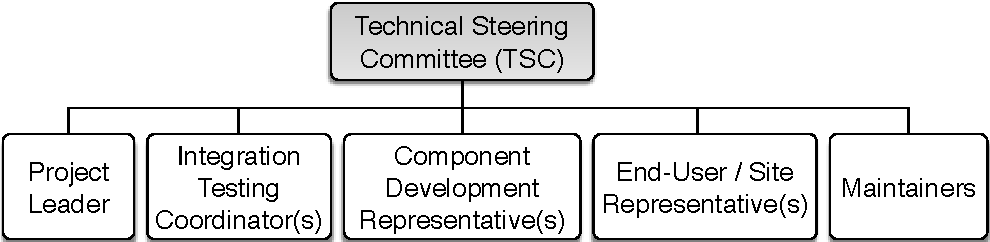
\includegraphics[width=1.0\linewidth]{figures/governance}
  \caption{Identified roles within the OpenHPC Technical Steering Committee (TSC).}
  \label{fig:tsc_governance}
\end{figure}

\subsection{Installation/Repository Overview}
\label{sec:repo_enable}

As mentioned previously, OpenHPC endeavors to adopt a repository-based delivery
model similar to the underlying OS distributions commonly used as the basis for HPC
Linux clusters.  At present, OpenHPC is providing builds targeted against two
supported OS distributions: CentOS7 and SLES12. The underlying package
managers for these two distributions are {\bf \texttt yum} and {\bf \texttt zypper},
respectively, and OpenHPC provides public repositories that are compatible with
these RPM-based package managers.

The installation procedure outlined in current OpenHPC recipes targets
bare-metal systems and assumes that one of the supported base operating systems
is first installed on a chosen {\em master} host. This is typically done
leveraging bootable media from ISO images provided by the base OS and once
installed, OpenHPC recipes highlight steps to install additional software and
perform configurations to use the {\em master} host to provision the remaining
cluster.

\newpage
An overview of the physical infrastructure expected for use with
current OpenHPC recipes is shown in
Figure~\ref{fig:cluster_arch} and highlights the high-level networking
configuration. The {\em master} host requires at least two Ethernet interfaces
with {\em eth0} connected to the local data center network and {\em eth1} used
to provision and manage the cluster backend (these interface names
are examples and may be different depending on local settings and OS
conventions). Two logical IP interfaces are expected to each compute node: the
first is the standard Ethernet interface that will be used for provisioning and
resource management. The second is used to connect to each host's baseboard
management controller (BMC) and is
used for power management and remote console access. Physical connectivity for
these two logical IP networks is often accommodated via separate cabling and
switching infrastructure; however, an alternate configuration can also be
accommodated via the use of a shared NIC.
%, which runs a packet filter to divert
%management packets between the host and BMC.
For power management, we assume that the compute node 
BMCs are available via IPMI from the chosen master host. For file
systems, the current recipe(s) document setting up the chosen master
host as an NFS file system that is made available to the compute
nodes. Installation information is also discussed to optionally include a
Lustre~\cite{Lustre_url} file system mount.

\begin{figure}[h]
  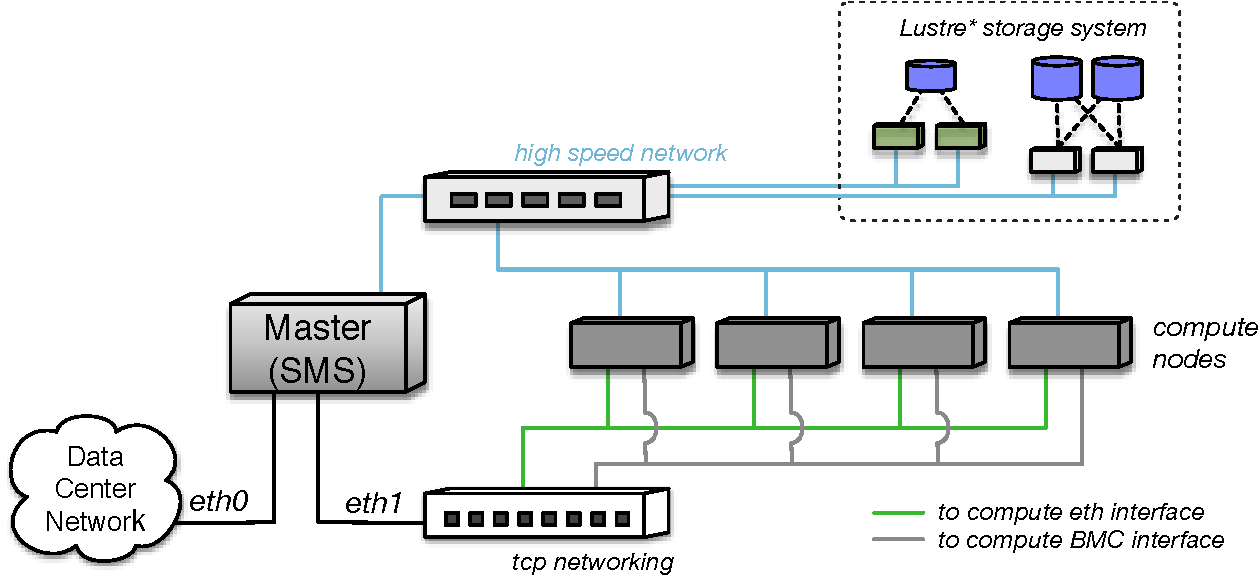
\includegraphics[width=0.95\linewidth]{figures/ohpc-arch-small.pdf}
  \caption{Overview of physical cluster infrastructure expected with OpenHPC
    installation recipes.}
  \label{fig:cluster_arch}
\end{figure}

\noindent{\bf Community Repo:} In cases where external network connectivity is
available on the {\em master} host, OpenHPC provides an \texttt{ohpc-release}
package that includes GPG keys for package signing and repository enablement.
This package can be downloaded from the OpenHPC GitHub community site directly
(\url{https://github.com/openhpc/ohpc}). Note that additional repositories may
be required to resolve package dependencies and, in the case of CentOS, access
to the EPEL~\cite{epel_url} repo is currently required.

The most recent release branch for OpenHPC is version~1.1 and the output in
Figure~\ref{fig:repolist} highlights the typical repository setup after
installation of the \texttt{openhpc-release-1.1} RPM in a CentOS
environment. Following typical OS distro conventions, two OpenHPC
repositories are enabled by default: a { \bf base} repo corresponding to the
original 1.1 release and an {\bf updates} repo that provides rolling fixes and
enhancements against the 1.1 tree.

\begin{figure}[h]
\begin{lstlisting}[language=bash,keywords={}]
(*\#*) yum repolist
repo id              repo name
OpenHPC              OpenHPC-1.1 - Base
OpenHPC-updates      OpenHPC-1.1 - Updates
base                 CentOS-7 - Base
epel                 Extra Packages for Enterprise...
\end{lstlisting}
\vspace*{-0.3cm}
  \caption{Typical package repository configuration after enabling OpenHPC
    (CentOS example).}
    \label{fig:repolist}
\end{figure}

\subsection{Packaging} \label{sec:packaging}

%Being building-block oriented in nature,
To highlight several aspects of the current packaging conventions, we next
present several installation examples. Note that this
discussion does not endeavor to replicate an entire install procedure, and
interested readers are invited to consult the latest installation recipe(s) that
are available on the community GitHub site (or via the installable
\texttt{docs-ohpc} RPM) for more detailed instructions.

Once the OpenHPC repository is enabled locally, a range of packages are
available and a typical install on the {\em master} host begins with the
installation of desired system administration services. In the example that
follows, the Warewulf provisioning system~\cite{warewulf_url} and SLURM
resource manager is installed using available convenience groups:

\begin{figure}[h]
\begin{lstlisting}[language=bash,keywords={}]
[sms](*\#*) yum -i groupinstall ohpc-warewulf
[sms](*\#*) yum -i groupinstall ohpc-slurm-server
\end{lstlisting}
\vspace*{-0.3cm}
  \caption{Example installations using convenience groups.}
    \label{fig:grouplinstall}
\end{figure}
  
Convenience groups like the examples above are prefixed with the ``ohpc-'' tag
and install a collection of related packages. As an example, the
\texttt{ohpc-warewulf} group expands to include all the packages needed to
enable a Warewulf provisioning server. Similarly, the
\texttt{ohpc-slurm-server} group includes the packages needed to stand up a
SLURM control daemon for resource management~\cite{Jette02slurm:simple} across
the cluster.  Although not shown here, a related \texttt{ohpc-slurm-client}
group is also available to allow for installation of a smaller set of packages
needed to enable a SLURM client (typically installed in compute node images).

Note that individual packages provided via OpenHPC have their names appended
with the ``ohpc'' suffix.  The motivation for this convention was to allow for
easy wild-carding queries with package managers, and to also provide the
ability to install OpenHPC-packaged versions of software alongside of alternate
distro versions of the same packages (if available).  Finally, while the
examples here continue to use the \texttt{yum} package manager, equivalent
commands can be substituted using \texttt{zypper} when using SLES.  \\

\noindent {\bf Development Libraries}: In addition to providing tools primarily
targeted at system administrators, OpenHPC also provides pre-packaged builds
for a number of popular open-source tools and libraries used by HPC
applications and developers. For example, OpenHPC includes a variety of builds
for FFTW~\cite{FFTW05} and HDF5~\cite{hdf5_url} (including serial and
parallel I/O support), and the GNU Scientific Library (GSL). A number of other
development tools and libraries are included and the installation recipe(s)
contain a detailed package manifest highlighting what is available for a given
release. Note also that the list is expected to evolve
and expand over time as additional software components are integrated within
future releases.

General purpose HPC systems often rely on multiple compiler and MPI family
toolchains~\cite{tacc_sc_best_practices:2011} and OpenHPC supports this
strategy via the adoption of a hierarchical build configuration that is
cognizant of the need to deliver unique builds of a given software package for
each desired compiler/MPI permutation.
% Additional discussion on the build procedure will be highlighted in OBS section.
%%% Again, multiple builds of
%%% each package are available in the OpenHPC repository to support multiple
%%% compiler and MPI family combinations where appropriate.
The general naming convention for builds that have these toolchain dependencies 
%provided by OpenHPC
is to append the compiler and MPI family name that the
library was built against directly into the package name. For example,
libraries that do not require MPI as part of the build process adopt the
following RPM naming scheme: \\

\noindent
\texttt{package-<comp\_fam>-ohpc-<ver>-<rel>.rpm} \\

\noindent where \texttt{<comp\_fam>} maps to the underlying compiler family and \texttt{<ver>}
and \texttt{<rel>} correspond to the individual software version and build
release number, respectively.
Expanding on this convention, packages that also require MPI as part of the build 
additionally include the MPI family (\texttt{<mpi\_fam}>) name as follows: \\

\noindent
\texttt{package-<comp\_fam>-<mpi\_fam>-ohpc-<ver>-<rel>.rpm} \\

\noindent
Given the large number of installation permutations possible for software
supporting multiple compiler/MPI toolchains, combined with the fact that HPC
sites also tend to make multiple versions of a particular component available
to their users, there is a clear need to support a flexible development environment for end
users. A popular historical choice in this space over the years has been the
use of Environment Modules~\cite{furlani_1996} to expose a \texttt{modules}
command within a user's shell environment allowing them to load/unload desired
software packages via management of key environment variables
(e.g. \texttt{{PATH}} and \texttt{{LD\_LIBRARY\_PATH}}). Several
implementations of the modules system have evolved and OpenHPC leverages a
recent variant named {\em Lmod}~\cite{tacc_sc_best_practices:2011,lmod_url}
which is Lua-based, and has embedded support for managing the
hierarchical software matrix adopted in OpenHPC.  In addition to providing a
pre-packaged build of {\em Lmod}, development libraries and tools integrated
within OpenHPC include the installation of companion module files.
%for use with
%{\em Lmod}.
Consequently, once a desired package is installed, end users can then access
and query the software through the underlying modules system. The packaging
process includes a consistent set of environment variables for users to
access a particular package's path for available header files and dynamic
libraries. As an example, consider the following installation of the
PETSc~\cite{PETSc_url} scientific toolkit built using the GNU compiler and
MVAPICH2~\cite{mvapich2} MPI toolchain.

\begin{figure}[h]
\begin{lstlisting}[language=bash,keywords={}]
[sms](*\#*) yum install petsc-gnu-mvapich2-ohpc
\end{lstlisting}
\vspace*{-0.3cm}
  \caption{Installation of PETSc for a particular compiler/MPI combination.}
    \label{fig:petscinstall}
\end{figure}

\noindent
Next, assume an end user has a simple C code example they wish to build against
the installed PETSc version. This can be accomplished as follows by leveraging
the environment variables enabled through loading of the provided module file:

\begin{figure}[h]
\begin{lstlisting}[language=bash,keywords={},literate={-}{-}1]
joeuser (*\$*) module load petsc
joeuser (*\$*) mpicc -I$PETSC_INC petsc_hello.c \
             -L$PETSC_LIB -lpetsc
\end{lstlisting}
\vspace*{-0.3cm}
  \caption{Example compilation using variables provided by PETSc module file.}
    \label{fig:petsccompile}
\end{figure}

\newpage
Owing to the hierarchical capabilities of {\em Lmod}, if multiple PETSc
permutations were installed (e.g. for different MPI toolchains), the end user
would also be able to swap toolchains and the underlying modules system will
automatically update the user's environment accordingly to be consistent with
the currently loaded MPI family.

%\subsection{Conventions}
%\subsubsection{Architecture}
%%We have assembled a variety of common ingredients required to deploy and manage 
%%an HPC Linux cluster including provisioning tools, resource management, I/O 
%%libraries, development tools, and a variety of scientific libraries. The 
%%delivery mechanism is via standard package managers (i.e., there are public 
%%OpenHPC repositories for both yum and zypper). OpenHPC currently supports CentOS
%%7 and SUSE's SLE 12. A single RPM spec file generates packages for both base
%%operating systems. This multiple target model also extends to compiler
%%toolchains and MPI runtime libraries. For some components that means a spec file
%%can generate 12 different versions of a package. This complexity is masked by
%%yum/zypper convenience groups, macros within the build system, and hierarchical 
%%Lmod environment modules for users.


%--example showing convenience group installation, package name convention, module
%load--

% - repo layout description

\subsection{Build Infrastructure} \label{sec:build_infra}

To provide the public package repositories highlighted previously in
\S\ref{sec:repo_enable}, OpenHPC utilizes a set of standalone resources
running the Open Build Service (OBS)~\cite{OBS_url}.  OBS is an open-source
distribution development platform written in Perl that provides a transparent
infrastructure for the development of Linux distributions and is the underlying
build system for openSUSE.  The public OBS instance for OpenHPC is available at
\url{https://build.openhpc.community}.

While OpenHPC does not, by itself, provide a complete Linux distribution, it
does have in common many of the same packaging requirements and targets a
delivery mechanism that adopts Linux sysadmin familiarity.  OBS aids in this
process by driving simultaneous builds for multiple OS distributions (e.g. 
CentOS and SLES), multiple target architectures (e.g. x86_64 and aarch64),
and by performing dependency analysis among components, triggering downstream
builds as necessary based on upstream changes. Each build is carried out in a
Qemu-KVM environment for repeatability, and OBS manages publication of the resulting
builds into package repositories compatible with {\texttt yum} and {\texttt
  zypper}. Both binary and source RPMs are made available as part of this process.

The primary inputs for OBS are the instructions necessary to build a particular
package, typically housed in an RPM .spec file. These .spec files are version controlled in the
community GitHub repository and are templated in a way to have a single input
drive multiple compiler/MPI family combinations.  To illustrate this approach,
the code in Figure~\ref{fig:metis_spec} highlights a small portion from the .spec file used to build
METIS~\cite{Karypis:1998}, a popular domain decomposition library. The primary
item of note is the the use of a \texttt{compiler\_family} macro which defaults
to the gnu compiler family if not specified otherwise.  This variable is then used
to decide on underlying build and installation requirements chosen to match the
desired runtime.

\begin{figure}[h]
%  \begin{lstlisting}[language=bash,keywords={},basicstyle=\scriptsize\ttfamily,keepspaces]
\begin{lstlisting}[language=bash,keywords={},basicstyle=\fontsize{7.8}{10}\ttfamily,keepspaces]
%{!?compiler_family: %define compiler_family gnu}

(*\#*) Compiler dependencies
BuildRequires: lmod%{PROJ_DELIM}
%if %{compiler_family} == gnu
BuildRequires: gnu-compilers%{PROJ_DELIM}
Requires:      gnu-compilers%{PROJ_DELIM}
%endif
%if %{compiler_family} == intel
BuildRequires: gcc-c++ intel-compilers-devel%{PROJ_DELIM}
Requires:      gcc-c++ intel-compilers-devel%{PROJ_DELIM}
%endif
\end{lstlisting}
\vspace*{-0.3cm}
  \caption{Snippet from METIS .spec file highlighting compiler hierarchy
    template used during the build process.}
    \label{fig:metis_spec}
\end{figure}

To link the underlying source and build infrastructure together, OpenHPC's public OBS
instance is integrated with the associated GitHub repository. A benefit of
this integration is that whenever commits are made on key git branches,
OBS automatically triggers corresponding package rebuilds. OBS also analyzes
inter-package dependencies and downstream packages are rebuilt as well with
updated packages published after all builds are completed.

For builds that require MPI linkage, a companion .spec template is used which
adds an \texttt{mpi\_family} variable that defaults to the
OpenMPI~\cite{gabriel04:openmpi} stack unless specified otherwise.  To
maintain the concept of having a single maintainer commit drive multiple
builds, our OBS configuration leverages the ability to {\em link} related software
packages together. To illustrate this process, the text in
Figure~\ref{fig:obs_link} contains the underlying
OBS package configuration syntax for the PETSc toolkit built against
MVAPICH2. The top line indicates that the MVAPICH2-based build is simply a link
to the parent (default) package configuration that is OpenMPI based.  What
follows after that are stanzas that tell OBS to apply patches to the resulting
.spec file prior to doing a build. In this case, the patches are trivial and
simply redefine the \texttt{compiler\_family} and \texttt{mpi\_family} variables at
the top of the .spec file.  This linkage provides a convenient mechanism to
extend the hierarchical runtime family approach to the underlying build system.

\begin{figure}[h]
\begin{lstlisting}[language=bash,keywords={},basicstyle=\fontsize{7.8}{10}\ttfamily,keepspaces]
(*\#*) cat petsc-gnu-mvapich2/_link
<link project='OpenHPC:1.1' package='petsc-gnu-openmpi'>
<patches>
<topadd>%define compiler_family gnu</topadd>
<topadd>%define mpi_family mvapich2</topadd>
</patches>
</link>
\end{lstlisting}
\vspace*{-0.3cm}
\caption{Underlying OBS package config highlighting linkage between builds
  using different runtime hierarchies.}
\label{fig:obs_link}
\end{figure}

\subsection{Integration Testing} \label{sec:integ_testing}
To facilitate validation of the OpenHPC distribution as a whole, we have
devised a standalone integration test infrastructure. In order to exercise the
entire scope of the distribution, we first provision a cluster from bare-metal
using installation scripts provided as part of the OpenHPC documentation. Once
the cluster is up and running, we launch a suite of tests targeting the
functionality of each component. These tests are generally
pulled from component source distributions and aim to insure development
toolchains are functioning correctly and to ensure jobs perform under the
resource manager. The intent is not to replicate a particular component's own
validation tests, but rather to ensure all of OpenHPC is functionally
integrated. The testing framework is publicly available in the OpenHPC GitHub
repository.

A Jenkins continuous integration server~\cite{jenkins_url} manages a set of 
physical servers in our test infrastructure. Jenkins periodically kickstarts a cluster 
master node using out-of-the-box base OS repositories, and this master is then 
customized according to the OpenHPC install guide. The \LaTeX\ source for the 
install guide contains markup that is used to generate a \texttt{{bash}} script 
containing each command necessary to provision and configure the cluster and install OpenHPC
components. Jenkins executes this script, then launches the component test suite.

The component test suite relies on a custom autotools-based framework.
Individual runs of the test suite are customizable using familiar autoconf
syntax, and \texttt{{make check}} does what one might expect. The framework
also allows us to build and test multiple binaries of a particular component
for each permutation of compiler toolchain and MPI runtime if applicable.  We
utilize the Bash Automated Testing System (BATS)~\cite{bats_url} framework to
run tests on the cluster and report results back to Jenkins. An example test
driver shell script for the PETSc toolkit is highlighted in Figure~\ref{fig:test_loop}. Recall that this package
requires MPI linkage and the script highlights the fact that multiple tests are
performed for each supported compiler and MPI toolchain.

\begin{figure}[t]
\begin{lstlisting}[language=bash,keywords={},keepspaces]
(*\#*)!/bin/bash

status=0
cd libs/petsc || exit 1
export BATS_JUNIT_CLASS=PETSc

(*\#*) bootstrap the local autotools project 
./bootstrap || exit 1

for compiler in $COMPILER_FAMILIES ; do
    for mpi in $MPI_FAMILIES ; do

    echo "--------------------------------------"
    echo "Libraries: PETSc tests: $compiler-$mpi"
    echo "--------------------------------------"

    module purge          || exit 1
    module load prun      || exit 1
    module load $compiler || exit 1
    module load $mpi      || exit 1
    module load petsc     || exit 1

    ./configure           || exit 1
    make clean            || exit 1
    make -k check         || status=1

    save_logs_mpi_family tests $compiler $mpi

    make distclean
    done
done

exit ${status}
\end{lstlisting}
\vspace*{-0.3cm}
\caption{Example test driver script for PETSc.}
\label{fig:test_loop}
\end{figure}

As the test suite has grown over time to accommodate a growing set of integrated
components, the current test harness has both {\em short} and {\em long}
configuration options.  The short mode enables only a subset of tests in order
to keep the total runtime to approximately 10 minutes or less for more frequent
execution in our CI environment. For the most recent OpenHPC release, the long
mode with all relevant tests enabled requires approximate 90 minutes to complete
approximately 1,900 individually logged tests.


\section{Conclusions \& Future work}
This paper has presented an overview of OpenHPC, a collaborative Linux
Foundation project with organizational participation from academia, research
labs, and industry. The building-block nature of the OpenHPC repository was
highlighted along with some basic packaging conventions and an overview of the
underlying build and test infrastructure.

Future work by the OpenHPC Technical Steering Committee (TSC) is focused on
formalizing and publishing a component selection process by which the community
can request inclusion of additional software. Currently, OpenHPC provides simple
configuration recipes for HPC clusters, but future efforts will focus on 
providing automation for more advanced configuration and tuning to address
scalability, power management, and high availability concerns. We also hope to
expand community cooperation between complementary efforts by 
%continue driving standardization across the HPC landscape,
developing package dependency conventions with EasyBuild and Spack.
%Finally, we
%are working to deploy public continuous integration infrastructure, and
%enable corresponding builds and releases for the ARM architecture (aarch64).

%ACKNOWLEDGMENTS are optional
\section{Acknowledgments}

We would like to thank the Linux Foundation and associated members of the
OpenHPC collaborative project for supporting this community effort.  We are
particularly grateful to the additional members of the Technical Steering
Committee including Pavan Balaji, Todd Gamblin, Craig Gardner, Balazs Gerofi,
Jennifer Green, Douglas Jacobsen, Chulho Kim, Thomas Moschny, Craig Stewart,
and Scott Suchyta.
We are also grateful to donations
from Intel, Cavium, and Dell who have provided hardware to help support integration testing
efforts, and the Texas Advanced Computing Center for hosting OpenHPC infrastructure.


\bibliographystyle{abbrv}
\bibliography{hpcsyspros}


\end{document}
